% Compile with pdfLaTeX.
% Landscape version corresponding to the revised portrait template.
% Font matching is intentionally relaxed for this version.

\documentclass[a4paper,landscape]{article}

% Scroll down to line 74

% Minimal external packages:
\usepackage[a4paper,landscape,left=18mm,right=18mm,top=18mm,bottom=18mm]{geometry}
\usepackage{graphicx}
\usepackage{xcolor}
\usepackage{lipsum}
\usepackage{array}
\usepackage[T1]{fontenc}
\usepackage[sfdefault]{roboto}
\usepackage[
    colorlinks=true,
    urlcolor=blue,
    linkcolor=black,
    citecolor=blue
]{hyperref}

\pagestyle{empty}
\setlength{\parindent}{0pt}
\setlength{\parskip}{0pt}
\setlength{\tabcolsep}{0pt}
\definecolor{topicblue}{HTML}{2F5597}

% Lengths - specifications for template fonts, appearance
\newlength{\HeaderSize}
\setlength{\HeaderSize}{24pt}
\newlength{\HeaderSizeBaseline}
\setlength{\HeaderSizeBaseline}{28.8pt}

\newlength{\SectionSize}
\setlength{\SectionSize}{16pt}
\newlength{\SectionSizeBaseline}
\setlength{\SectionSizeBaseline}{1.2\SectionSize}

\newlength{\TextSize}
\setlength{\TextSize}{14pt}
\newlength{\TextSizeBaseline}
\setlength{\TextSizeBaseline}{1.3\TextSize}

\newlength{\CaptionSize}
\setlength{\CaptionSize}{12pt}
\newlength{\CaptionSizeBaseline}
\setlength{\CaptionSizeBaseline}{1.2\CaptionSize}

\newlength{\RefSize}
\setlength{\RefSize}{12pt}
\newlength{\RefSizeBaseline}
\setlength{\RefSizeBaseline}{1.4\RefSize}

\newlength{\vskipHeader}
\setlength{\vskipHeader}{8.0mm}
\newlength{\vskipSection}
\setlength{\vskipSection}{4.0mm}
\newlength{\vskipText}
\setlength{\vskipText}{2.0mm}
\newlength{\vskipImage}
\setlength{\vskipImage}{16.0mm}

% Landscape geometry.
% The left panel is square; the right panel uses the remaining width.
\newlength{\LeftPanel}
\setlength{\LeftPanel}{164mm}
\newlength{\PanelGap}
\setlength{\PanelGap}{18mm}
\newlength{\RightPanel}
\setlength{\RightPanel}{79mm}

% Do not change anything above this line!

\begin{document}
\noindent
\begin{tabular}{@{}p{\LeftPanel}@{\hspace{\PanelGap}}p{\RightPanel}@{}}

% ======================= LEFT SQUARE =======================
\parbox[t][\LeftPanel][t]{\LeftPanel}{%

% High page header
\begin{center}
  {\fontsize{\HeaderSize}{\HeaderSizeBaseline}\selectfont\color{topicblue}%
  %
  % Agnese will modify this; For now write your name and number your projects with 1 and 2
   Project Topic:\hspace{9mm} (Agnese 2)} 
\end{center}

\vspace{\vskipHeader}

% Main title
{\fontsize{\SectionSize}{\SectionSizeBaseline}\selectfont\bfseries 
%
% Title
Patchy particles in 2D
\par}
\vspace{\vskipSection}

% Abstract / project description --> adjust accordingly
{\fontsize{\TextSize}{\TextSizeBaseline}\selectfont
%
% Intro+Motivation
Patchy particles are colloidal particles whose surfaces contain specific interaction sites, or “patches,” allowing them to form directional and selective bonds. Despite the simplicity of the individual particles and their interactions, these systems can display rich collective behavior and self-assemble into a variety of complex structures.
\par

\vspace{\vskipText}
% In this project
In this project, you will investigate the dynamics of patchy particles in two dimensions. Particular attention can be given to the formation and breaking of bonds between interacting patches and to how these microscopic processes affect the resulting structures. The project may explore systems with different populations or types of patchy colloids, as well as the influence of complex or crowded environments. The goal is to understand how particle properties, interactions, and environmental conditions determine the dynamics and self-organization of patchy-particle systems.
\par
}

\vfill

% References are entered manually. No .bib file / BibTeX / biblatex.
{\fontsize{\SectionSize}{\SectionSizeBaseline}\selectfont\bfseries References: \par}
\vspace{\vskipSection}

{\fontsize{\RefSize}{\RefSizeBaseline}\selectfont
% 
% Reference 1
[1] Swinkels,  P. J. M. \textit{et al,} \textit{Networks of Limited-Valency Patchy Particles}, Phys. Rev. Lett. \textbf{132}, 078203 (2024).\\
\href{https://doi.org/10.1103/PhysRevLett.132.078203}{https://doi.org/10.1103/PhysRevLett.132.078203} 
\par
% 
}
\vspace{\vskipText}
}% end left square

&

% ======================= RIGHT COLUMN =======================
\parbox[t][\LeftPanel][c]{\RightPanel}{%
\centering
\ \\[3\vskipSection]
%
% Representative image + caption. 
\begin{tabular}{@{}c@{}}
%
% Image
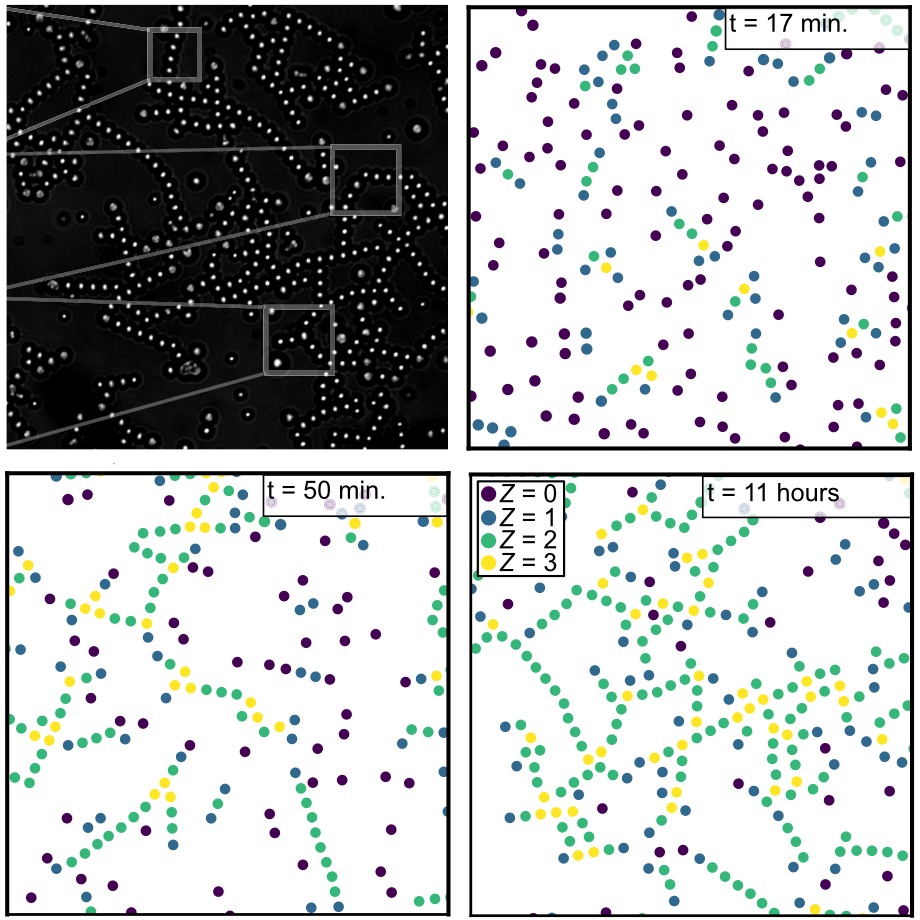
\includegraphics[width=\RightPanel]{patchycolloids.png}\\[\vskipSection] % name of the image 
\parbox{\RightPanel}{%
\fontsize{\CaptionSize}{\CaptionSizeBaseline}\selectfont
\textbf{Fig.1}\quad 
% 
% Title of the image (bold)
\textbf{Growth of colloidal network of divalent and pseudo-trivalent particles.} 
% 
% Body of the image caption.
Optical microscope image (top left) and reconstructions showing the evolution of the particle network (remaining panels). As time passes, linear chains becomes more defined as well as the formation of connecting nodes.
%
% Credits.
\textit{Image from Ref.~[1].} 
}
\end{tabular}
}% end right column

\end{tabular}
\end{document}
